\chapter{绪论}
本章旨在探讨长文本机器阅读理解的研究背景和意义,并对国内外研究现状的几个主要方面进行介绍,包括机器阅读理解、长文本机器阅读理解和开放域问答。
在此基础上,本章分析了关键科学问题和研究难点。
针对这些关键科学问题,本章详细介绍了本文的研究内容和组织结构。


\section{研究背景和意义}
机器阅读理解(Machine Reading Comprehension,简称MRC)旨在教会机器在理解给定自然语言文本的基础上回答与之相关的问题,一直是自然语言处理(Natural Language Processing,简称NLP)领域极具挑战性的前沿研究之一。

% 机器阅读理解的研究背景
早期的机器阅读理解主要依赖于浅层的自然语言处理技术\cite{Liu2019NeuralMR,Zhang2020MachineRC,Cui2019ASD},如关键词提取\cite{Li2021KeywordEM}、句法分析\cite{Yu2022SSAGNetSA}等,而这些技术忽略了句子之间的逻辑关系以及文本的语境信息。
这些技术可以用于对文本进行初步的处理和分析。

随着深度学习技术的发展,机器阅读理解的研究逐渐转向基于神经网络的方法\cite{hermann2015teaching}。
利用深度学习技术,可以构建端到端的模型,从而更好地捕捉句子之间的关系和语境信息,提高长文本机器阅读理解的准确率。

同时,计算机可以帮助人们自动化地理解和处理大量的文本信息,从而节省时间和精力。
这项技术也可以应用于很多场景,如自动化摘要\cite{Dong2018ASO}、文本分类\cite{Liu2016RecurrentNN}、信息检索\cite{Trabelsi2021NeuralRM}、知识图谱\cite{Lan2021KnowledgeGI}等任务,也可以在教育、医疗、金融、智能客服\cite{Ebersbach2016ArtificialNN}等领域使用,使人们能够更加高效的获取和利用信息。

% 长文本机器阅读理解的研究背景
随着数字化信息的快速发展,人们需要从各种各样的长文本中获取信息。
这包括但不限于新闻报道、学术论文、用户手册以及社交媒体。
但是,长文本中通常涵盖了丰富的信息和细节,这增加了人类理解和提取信息的难度。
因此,长文本机器阅读理解成为一项重要的研究任务,旨在通过计算机技术提高长文本处理的效率和准确性。

长文本机器阅读理解的研究与人工智能技术的发展密切相关。
随着深度学习技术在自然语言处理领域的广泛应用和不断发展,机器阅读理解的研究也取得了显著的进展。
深度学习技术为机器阅读理解任务提供了强有力的支持,使得研究人员可以通过大规模数据训练更加精准和高效的机器阅读理解模型。
这些模型可以有效地帮助人们处理长文本中的信息,从而提高信息处理的效率和准确性。

因此,长文本机器阅读理解的研究背景涉及到多个方面,包括人们对于高效阅读的需求、处理复杂语义的挑战以及深度学习技术的快速发展等。
这些方面共同推动着长文本机器阅读理解的不断发展和进步,使得机器能够更好地理解和处理长文本中的信息。
随着这些领域的不断发展和完善,长文本机器阅读理解技术将在未来得到更加广泛的应用,并且在各个领域中发挥着越来越重要的作用。


\section{国内外研究现状}
本节将从机器阅读理解、长文本机器阅读理解以及开放域问答三个研究视角出发,全面介绍国内外关于面向长文本机器阅读理解任务的相关研究工作。

\subsection{机器阅读理解}
机器阅读理解\cite{hermann2015teaching}是自然语言处理领域的研究热点,近年来在国内外都得到了广泛的关注和研究。

% 国外研究现状
随着各种深度学习技术的引入,机器阅读理解在近年来得到了越来越多的关注和发展。
% 数据集
% SQuAD
早在2015年,斯坦福大学推出了首个个由自然语言问题构成的的大规模机器阅读理解数据集SQuAD\cite{rajpurkar2016squad};
SQuAD数据集的目标是让机器阅读理解模型能够回答自然语言问题,并从给定的篇章中正确地提取出答案。
% SQuAD2.0
继SQuAD数据集之后,研究者们陆续提出了更多具有挑战性的大规模机器阅读理解数据集。
为了提升模型回答的能力,SQuAD2.0\cite{Rajpurkar2018KnowWY}横空出世;
相比于SQuAD,增加了一些负样本,这些负样本包括了那些在篇章中无法找到答案的问题;
因此,SQuAD2.0不仅要求模型回答问题,还需要模型能够判断出问题是否有答案。
% NewsQA
NewsQA\cite{trischler2016newsqa}也是一个类似于SQuAD的大规模机器阅读理解数据集,专注于新闻文章的阅读理解,其中包括来自CNN和Daily Mail等新闻网站的超过10,000篇新闻文章。
% RACE
此外,多项选择式机器阅读理解数据集RACE\cite{lai2017race},类似于中国学生参加的中考和高考英语,收录了来自高中和大学英语考试中的阅读理解题目;
RACE数据集中的问题包含多种类型,涵盖了不同难度级别,既有简单的词汇理解,也有复杂的推理和推断。
% HotpotQA
基于多跳推理的大规模机器阅读理解数据集HotpotQA\cite{Yang2018HotpotQAAD},要求模型搜索多个文档的信息,回答一系列问题;
由于涉及多个文档信息,HotpotQA需要模型进行多文档联合推理。

% 模型
与此同时,伴随着大规模机器阅读理解数据集的问世,基于神经网络的机器阅读理解模型也相继涌现。
基于神经网络的机器阅读理解模型大多采用嵌入层,编码层,交互层和输出层等四层架构。
% BiDAF
BiDAF\cite{Seo2016BidirectionalAF}最早实现了双向注意力流机制,将问题与文本之间的语义关联性建模为一个注意力矩阵;
并且通过引入字符级别的编码器,增强了模型对于语言的理解能力和语义建模能力。
% Reasonet
基于知识图谱的机器阅读理解模型Reasonet\cite{Shen2016ReasoNetLT},通过将知识图谱中的实体和关系引入到机器阅读理解模型中,来提高模型的推理能力和文本理解能力。
% QANet
基于卷积神经网络的QANet\cite{Yu2018QANetCL},使用自注意力机制来学习文章和问题之间的交互表示,捕捉文章中与问题相关的信息,从而更有效的处理长文本和多文档场景。
这些模型大多基于深度学习技术,通过对大规模数据的学习来提高阅读理解的能力。
% Match-LSTM
此外,基于多层LSTM的模型Match-LSTM\cite{Wang2016MachineCU},可以同时对上下文和问题进行建模,并使用注意力机制来对匹配信息进行加权。
% BERT
在Transformer架构发布之后,研究人员陆续提出了各种预训练语言模型,例如BERT\cite{devlin2018bert}、RoBERTa\cite{liu2019roberta}、DeBERTa\cite{he2021debertav3}等,并在各种机器阅读理解任务上取得了成功。
这些预训练语言模型极大地推进了自然语言处理领域的发展,它们的成功很大程度上归功于它们能够通过对大规模语料库的无监督预训练学习到文本的丰富表示。
因此,本文提出的面向长文本的机器阅读理解方法均基于预训练语言模型进行开研究与开发。

% 国内研究现状
与此同时,国内研究者在机器阅读理解领域也取得了一定的进展。
% 数据集
一些国内高校和科研机构也相继推出了机器阅读理解数据集和模型。
% 清华大学
清华大学自然语言处理与社会人文计算实验室提出的中文机器阅读理解数据集CMRC\cite{Cui2019ASD},涵盖了新闻、百科、论坛等不同类型的文本,同时考虑了答案的多样性和篇章的连贯性。
% 百度
百度提出的中文机器阅读理解数据集DuReader\cite{He2017DuReaderAC},囊括了答案抽取问题,以及选择题;
该数据集在答案抽取和篇章连贯性方面的研究具有重要意义。
% 华为
华为也针对汉语语言提出了CLUER-MRC\cite{xu2020clue}等四个相关的中文机器阅读理解数据集。

% 方法
除了数据集的构建外,中文机器阅读理解方面的研究还包括了一系列的方法探索和技术创新。
% Chinese Machine Reading Comprehension Based on Language Model Containing Knowledge
Wentong\ Chen等人\cite{Chen2022ChineseMR}提出了一种利用预训练的语言模型来提高中文机器阅读理解性能的方法,同时考虑了人类在理解文本时会关联的一些外部相关知识;
该工作在BERT模型的基础上,引入了一个知识库模块,用于从给定的问题和上下文中抽取相关知识,并将其融合到语言模型中。
% Machine Reading Comprehension Model Based on Multi-head Attention Mechanism
Xue等人\cite{xue2022machine}提出了一种基于多头注意力机制的机器阅读理解模型,能有效的捕捉中文文本和问题之间的关系。


\subsection{长文本机器阅读理解}
长文本机器阅读理解是在机器阅读理解的基础上,把输入文本换成了更长的形式。
长文本阅读理解需要更强的对上下文和语境的理解能力,并且需要解决长文本中的信息丰富性、篇章结构复杂等挑战。
如今,国内外研究者们都在积极探索这个问题,并取得了一些进展。

% 数据集
% TriviaQA
TriviaQA\cite{Joshi2017TriviaQAAL}是一个长文本机器阅读理解数据集,其问题和文本来自于维基百科、Web网页等多个知识来源,文本长度有很大的变化范围,短至几百个单词,长可达几千甚至上万个单词;
该数据集的发布推动了长文本机器阅读理解任务的研究,并成为该领域研究的重要基准数据集之一。
% NarrativeQA
NarrativeQA\cite{Kocisk2017TheNR}是一个包含大量小说和电影剧本的数据集,用于自然语言处理和长文本机器阅读理解研究。

% 国内外研究现状
% 滑动窗口
关于长文本的处理方法,滑动窗口\cite{joshi2019bert}机制是一种常用的技术,它将长文本分割成多个较小的片段,以便于模型处理。
% A Thorough Examination of the CNN/Daily Mail Reading Comprehension Task
Danqi\ Chen等人\cite{Chen2016ATE}最早使用滑动窗口技术将长篇新闻文章分成多个段落,然后使用卷积神经网络模型进行阅读理解。
% Machine Comprehension Using Match-LSTM and Answer Pointer
随后,滑动窗口技术被广泛应用于长文本机器阅读理解任务中。
例如,Shuohang Wang等人\cite{Wang2016MachineCU}将长文本切分成多个窗口,并使用基于LSTM和注意力机制的模型来处理每个窗口,最终预测答案。
% R-Net: Machine Reading Comprehension with Self-Matching Networks
Wang Wenhui等人\cite{wang2017r}也采用滑动窗口技术来处理长文本,然后使用自匹配注意力网络\cite{Wang2017GatedSN}(Self-matching Networks)来捕捉文本之间的交互信息。
% DPR
除了这种方法,Facebook AI Research在2018年提出了稠密向量检索\cite{Karpukhin2020DensePR}(Dense Passage Retrieval, 简称DPR),它是一种从大规模文本集合中检索出最相关的文本段落的检索技术;
DPR利用双塔结构将文本表示为向量,并通过检索候选文本库的方式来处理长文本机器阅读理解问题。
此后,DPR被广泛应用于TriviaQA,Natrual Questions等多个数据集,并取得了很好的效果。
% Transformer-XL
此外,Transformer-XL\cite{Dai2019TransformerXLAL}在基于Transformer\cite{vaswani2017attention}语言模型的基础上,引入了递归机制和相对位置编码来解决长文本的问题;
递归机制允许模型在处理长序列时保留之前的状态信息;
相对位置编码技术允许模型在处理长文本时捕捉到相对位置的信息。
% CogLTX
国内研究者们也在长文本机器阅读理解领域进行了很多探索和实践。
清华大学和阿里巴巴联合提出了一种基于认知理论的框架CogLTX\cite{Ding2020CogLTXAB},可以将BERT等预训练语言模型应用到长文本上;
CogLTX通过训练一个判断模型来识别长文本中的关键句子,并将其串接进行推理,并通过排练和衰减实现多步骤推理。


\subsection{开放域问答}
开放域问答\cite{allam2012question}(Open Domain Question Answering)是一种自然语言处理任务,旨在从大规模的自由文本中回答人类提出的自然语言问题。
它通常包含信息检索和阅读理解两个子任务。
由于其自由文本的语言表达方式和信息组织方式多样,开放域问答技术通常要求模型具有对多样化文本的理解、推理和组织能力。
开放域问答技术通常可以用于搜索引擎当中,如今很多国内外学者都在研究这一技术的应用与创新。

% 数据集
% Natural Question
Natural Questions\cite{Kwiatkowski2019NaturalQA}(NQ)是由Google推出的一个开放域问答数据集,它是一个基于真实用户提问和真实网页文本的数据集;
NQ信息检索任务要求系统仅通过问题,从真实网页中选择一个最相关的文档。
% SearchQA
SearchQA\cite{Dunn2017SearchQAAN}是一个基于搜索引擎的开放域问答数据集,其中由超过140,000个人工制作的问题来自于人们在真实的搜索引擎中提出的查询;
该数据集的特点是问题的多样性和复杂性,其中包括一些需要深入理解文化、历史和常识的问题。

% 国内外研究现状
% Open Domain Question Answering Using Early Fusion of Knowledge Bases and Text
% Pipeline方法作为最早针对开放域问答的方法,类似搜索引擎的工作原理,将开放域问答分为Query理解,候选召回和答案抽取等部分。
Dheeraj Rajagopal等人\cite{Sun2018OpenDQ}提出了一种Pipeline的方法,来解决开放域问答任务中的挑战。
具体来说,该方法首先使用TF-IDF\cite{SprckJones2021ASI}等技术对文本进行编码,然后使用知识库中的实体和属性对编码进行扩展,以便更好地捕获问题和答案之间的语义关系;
接下来,该方法使用文本和知识库中的信息进行匹配和排序,并使用基于规则和基于机器学习的技术来生成答案。
% Reading Wikipedia to Answer Open-Domain Questions
另一种称为“两阶段方法”的流程是,首先使用检索器对大量给定的文档进行筛选,从中提取与问题相关的部分文本片段,然后从这些文本片段中抽取出答案。
Danqi Chen等人\cite{Chen2017ReadingWT}提出了一种新的方法,使用预训练语言模型来代替传统的阅读理解模型,对Wikipedia的文章进行阅读和理解,从中抽取问题相关的段落和答案。
% ORQA: Open Retrieval Question Answering
部分科研工作采用了端到端学习的方式,将检索器和阅读器模型同时进行训练,从而实现更加紧密的模型集成和协同工作。
其中一个典型例子是ORQA\cite{lee2019orqa},该方法通过联合训练检索器和阅读器,实现了对候选文档的精细筛选和对答案的精准抽取,从而提高了整个Pipeline的效率和准确性。
% How Much Knowledge Can You Pack Into the Parameters of a Language Model?
也有一些大模型,甚至可以不进行微调,而直接预测答案。
Adam Roberts等人\cite{Roberts2020HowMK}探讨了神经语言模型在无结构文本上训练时能够隐式地存储和检索知识的能力,并提出了一种评估方法来测量模型参数中包含的知识量。


\section{关键问题和研究难点}
机器阅读理解可以应用于多种自然语言处理任务,其具有重要的理论意义和广阔的应用前景。
如今,以预训练语言模型为主的神经机器阅读理解技术得到了快速发展,但机器阅读理解模型在长文本问答场景下仍有巨大的提升空间。

% 关键问题
长文本机器阅读理解的关键问题和研究难点主要包括以下几个方面:

% 问题理解
(1)问题理解

多文档机器阅读理解\cite{song2019multi}是长文本机器阅读理解的一种形式,其与传统的阅读理解任务相比,需要更深入的理解和推理。
该任务中问题的多跳形式使得问题的语法结构和包含的内容信息非常复杂,这使得神经网络模型在理解问题时面临许多挑战。
例如,模型需要理解问题中的关键信息和上下文,并能够识别问题中不同子问题之间的联系和顺序,以便逐步构建问题的完整解答。
问题理解的难点在于需要将自然语言转换为计算机可以理解的形式,同时还需要在不丢失关键信息的前提下对问题进行简化,以提高模型的理解能力。

为了解决这个问题,研究者们提出了各种不同的方法,包括基于图神经网络\cite{ding2019cogqa}的方法、基于知识库\cite{Luo2018KnowledgeBQ}的方法、基于语义\cite{zhang2021skeleton}的方法和基于转换\cite{Tu2019MultihopRC}的方法等。
这些方法都旨在提高模型对问题理解的能力,以实现更加准确和智能的多文档机器阅读理解。

% 段落或文档检索
(2)文档选择

在长文本机器阅读理解任务中,有时需要从大量的文档或段落中选择与问题相关的文档进行阅读理解。
如果直接将所有文档都送入神经网络模型进行处理,会导致计算代价过大,同时降低模型的准确性和鲁棒性。
因此,文档选择成为了长文本机器阅读理解任务中的一个关键问题,其目标是从候选文档集中快速且准确地筛选出与问题相关的文档,以减少计算代价和提高精度。

文档选择的难点在于如何有效地区分候选文档中与问题相关的内容和无关的内容。
这需要模型能够理解问题的意义和背景,并能够识别出文档中与问题相关的段落和句子。
现有的文档选择方法包括基于特征\cite{Severyn2015LearningTR}的方法、基于深度学习\cite{wu2017sequential}的方法和基于知识库\cite{Luo2018KnowledgeBQ}的方法等。
这些方法尝试从不同的角度对文档进行建模,以便更好地捕捉与问题相关的信息。
% 例如,基于深度学习的方法可以利用神经网络自动学习文档和问题之间的语义联系,而基于知识库的方法可以利用外部知识库中的知识来指导文档选择。
此外,研究者们还尝试了多阶段的文档选择\cite{Gan2019MultistepRV}方法,通过逐步缩小候选文档集的规模来提高文档选择的准确性和效率。

% 答案抽取
(3)答案抽取

机器阅读理解中的答案抽取是指如何从选出的相关段落中准确地抽取出符合问题要求的答案,以满足用户需求和提高质量。
% 其存在一些难点。
% 答案抽取是长文本机器阅读理解任务中的关键步骤之一,其目的是从选出的相关段落中准确地抽取出符合问题要求的答案。
这个过程不仅涉及到答案的位置定位,还需要对答案进行语义理解和答案类型判断等\cite{Zhou2021AnOD},以满足用户需求并提高阅读理解质量。

然而,答案抽取过程中存在一些难点。
首先,答案往往需要从复杂的文本结构中抽取,涉及到不同语言学层面的分析和理解,如词汇、句法和语义等\cite{Sordoni2015ANN,Moschitti2008KernelsOL,Thomas2022AnAH}。
这需要模型具备深厚的自然语言处理能力,能够理解文本中的逻辑关系和上下文信息,同时能够处理诸如命名实体识别和语义角色标注等任务\cite{Shi2019SimpleBM,Lample2016NeuralAF}。
其次,文本中可能存在歧义和多义性,同一问题可能有多个可能的答案,因此模型需要具备有效的答案排序和评估机制\cite{cui-etal-2020-multi}。
在答案抽取的过程中,模型还需要考虑多个相关段落中的答案,并进行合并和消歧。
最后,还需要考虑多种类型的问题,如开放式问题和封闭式问题等。
不同类型的问题对于答案抽取的难度和挑战也不同,因此需要针对不同类型的问题选择合适的答案抽取方法\cite{Zhang2016QuestionAO}。

% 总结
总之,长文本机器阅读理解是自然语言处理领域的一个重要研究方向,其涉及到多个复杂的子任务,如问题理解、文档选择、答案抽取等,每个子任务都存在着一些独特的难点和挑战。
解决这些难点不仅可以提高机器阅读理解的准确度和效率,还可以促进自然语言处理领域的发展。


\section{研究内容与组织结构}
针对以上总结出的关键问题与研究难点,本节首先引出本文的主要研究内容,随后给出文章的组织结构。

\subsection{研究内容}

% 整体任务结构
\begin{figure}
    \centering
    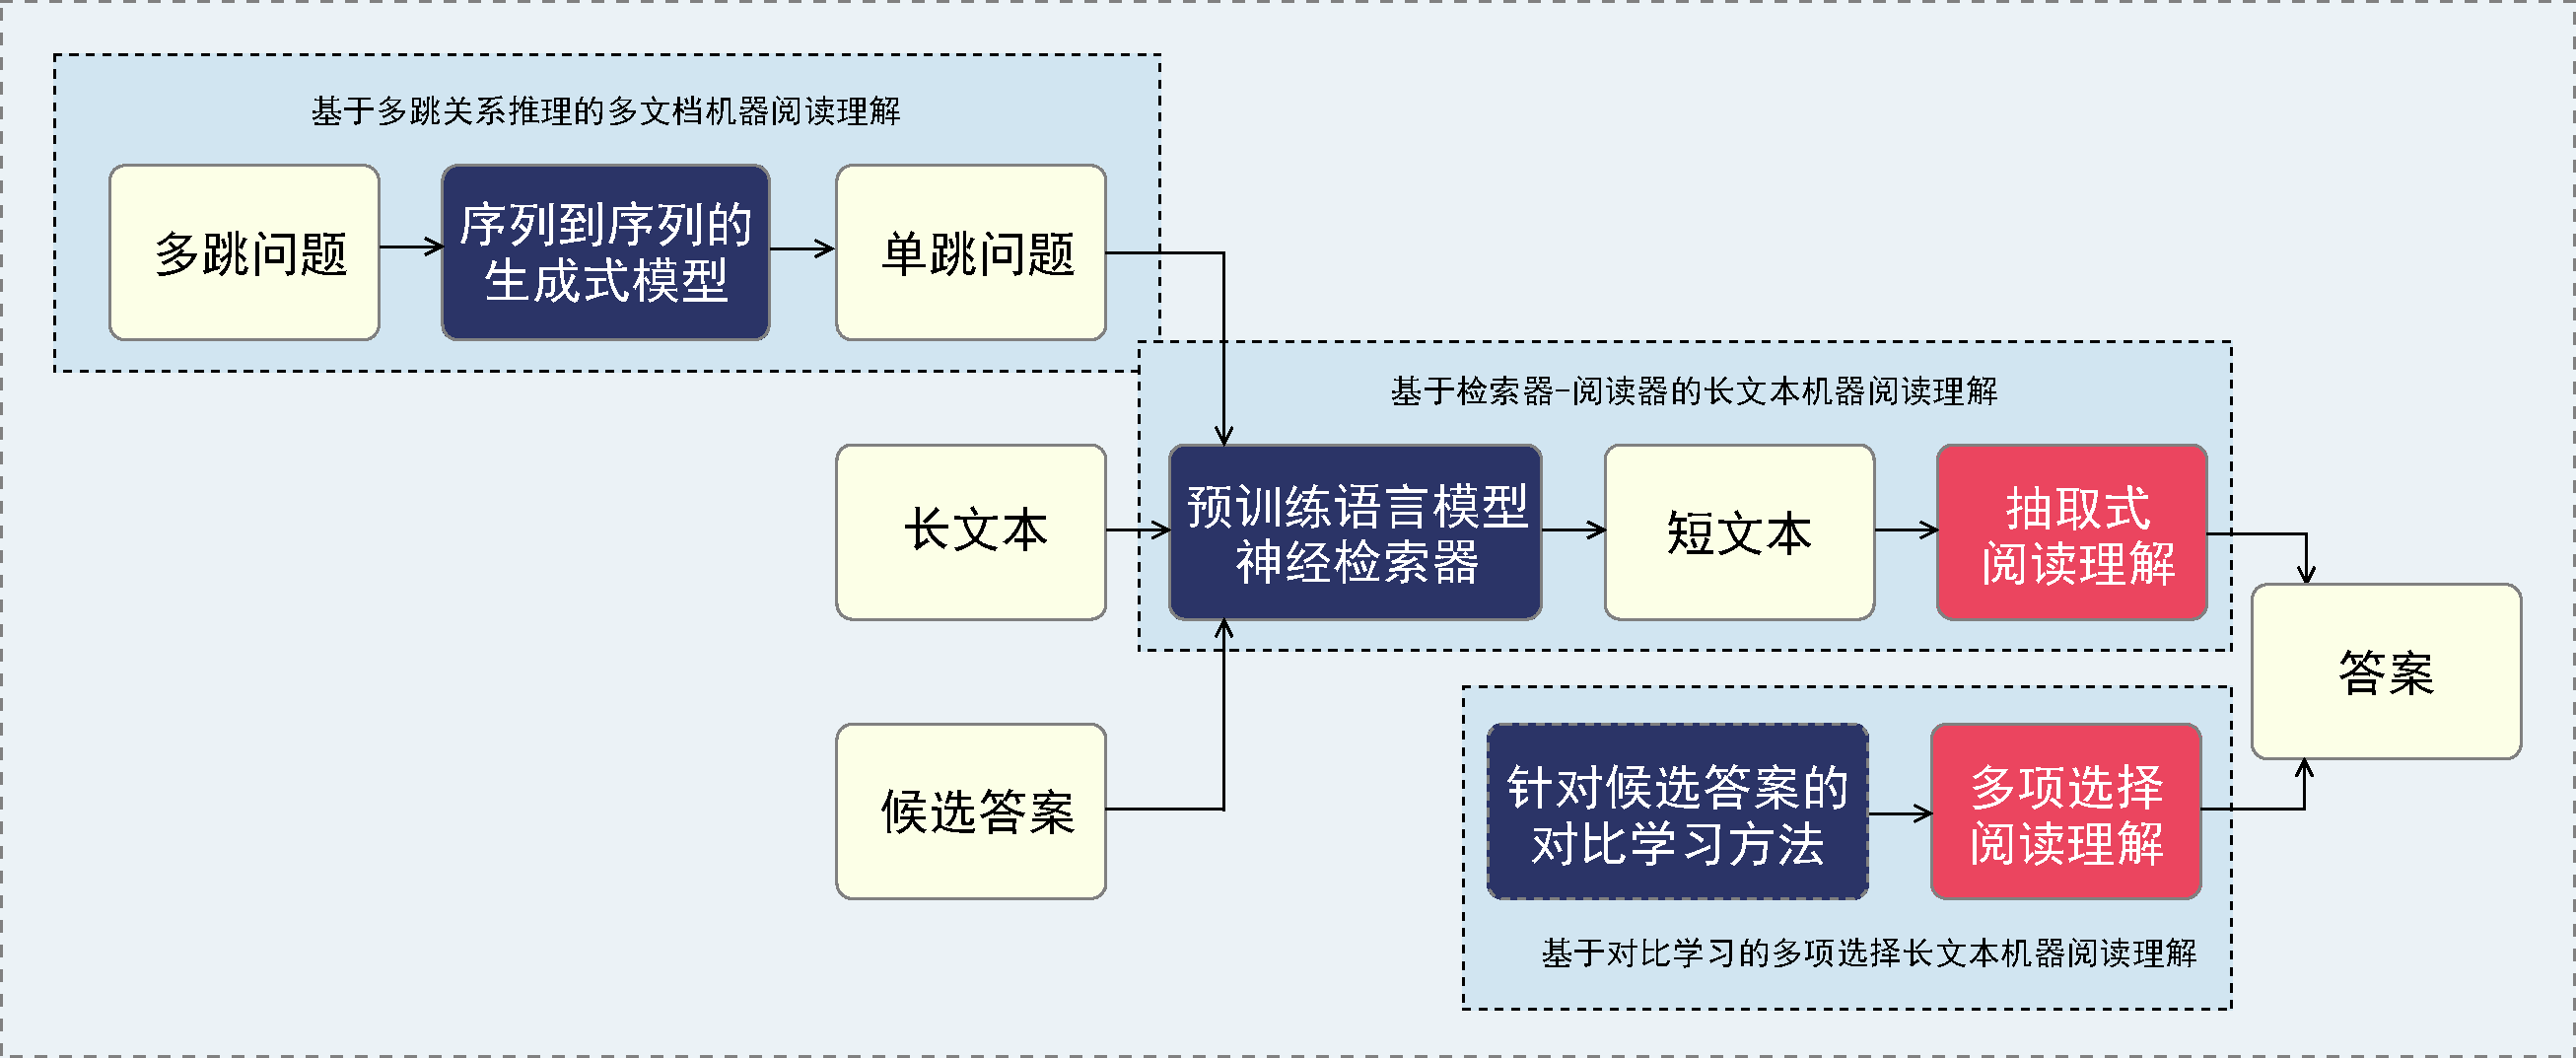
\includegraphics [width=1.0\textwidth] {figure/1-1.pdf}
    \caption{面向长文本的机器阅读理解研究框架图} 
    \label{fig:1-1}
\end{figure}


本文分别针对段落选择、多跳问题分解、答案选项融合等三个关键问题进行研究,对阅读理解模型进行改进。
针对上述关键问题,本文提出了一种面向长文本的机器阅读理解研究方法,其框架图如图~\ref{fig:1-1}~所示,具体分为以下三个方面:

% 面向新闻长文本的阅读理解研究
(1)基于检索器和阅读器段架构的长文本阅读理解研究

在长文本阅读理解任务中,传统的滑动窗口机制限制于每次只能处理512个词,难以建立长距离依赖,并且在截断部分时会丢失信息。
因此,本文提出了一种基于二阶段架构的解决方案,该方案首先选出证据,然后抽取答案片段。
在第一阶段中,检索器为每个文本片段打分,依据可回答性标签来对文本片段进行排序。
第二阶段中的阅读器从高置信文本片段堆中抽取答案。
这种方式可以在提取精炼信息的前提下进行答案抽取,缩小答案搜索范围,提高答案抽取的准确性。

% 基于问题分解的多跳长文本阅读理解研究
(2)基于问题分解的多跳长文本阅读理解研究

在多跳阅读理解任务中,由于问题过于复杂,且传统的机器阅读理解模型缺乏多跳推理能力,因此本研究提出了两种解决方案来将多跳问题分解为单跳问题。
第一种方法是使用序列到序列的生成式模型\cite{Lewis2019BARTDS,Ni2021SentenceT5SS}将多跳问题转化为多个单跳问题,并用检索模型和阅读理解模型分别筛选最佳文档,抽取最佳答案。
第二种方法是在每次生成当前问题时,利用前驱问题和前驱答案来引导生成过程,并通过检索模型和阅读理解模型抽取单跳问题的答案,直至遇到带有结束标志的单跳问题。
这两种方法可以有效地解决多文档阅读理解任务中的问题复杂性和推理能力缺失问题。

% 基于对比学习的多选长文本阅读理解研究
(3)基于对比学习的多项选择长文本阅读理解研究

在多项选择阅读理解任务中,由于部分干扰选项与正确选项在字面表述上过于相似,同时各个选项在编码阶段缺乏交互,因此存在着正确率偏低的问题。
为此,本文提出采用对比学习方法\cite{gao2021simcse},增强选项文本的编码表示能力,以提高选项的区分度;
同时利用样本内自注意力交互机制\cite{vaswani2017attention},建立多个选项之间的联系,从而使各个选项之间的编码能够相互影响,提高答案的准确性。

\subsection{组织结构}
本文共分为六个章节,论文组织结构和各个章节的主要内容如下:

% 第一章
第一章 绪论。
本章主要介绍长文本阅读理解研究的背景和意义,通过对国内外研究现状的分析,总结目前长文本阅读理解存在的问题和研究难点。
同时,本章还针对论文的研究内容和组织结构进行介绍。

% 第二章
第二章 任务定义和评价方法。
本章首先阐述了面向长文本的机器阅读理解任务的定义,并从样本分布和语言风格等角度对三个不同数据集进行了详细的实验语料资源分析,以此为基础对长文本机器阅读理解进行研究。
最后,本章对长文本阅读理解任务的性能评价指标进行了探讨。

% 第三章
第三章 基于检索器和阅读器架构的长文本阅读理解研究。
本章针对长文本阅读理解领域,提出了一种基于检索器-阅读器二阶段架构的方法。
该方法首先通过检索器,利用问题与文本片段之间的相关性,筛选出最有可能包含答案的一些文本片段。
接着,通过阅读器,采用当前比较先进的预训练语言模型,从这些精简后的文本片段中抽取最终的答案片段。

% 第五章
第四章 基于问题分解的多跳长文本阅读理解研究。
本章针对多跳阅读理解领域,提出了一种利用问题分解技术来简化问题的方法。
该方法通过使用序列到序列的生成式模型,将复杂的多跳问题分解为多个单跳问题。
然后,利用检索模型和阅读理解模型分别筛选出支持文档,并从中抽取最佳答案。

% 第四章
第五章 基于对比学习的多项选择长文本阅读理解研究。
本章针对多项选择长文本阅读理解领域,提出了一种以对比学习为主的研究方法。
该方法首先通过稠密向量检索的方式,从长文本中筛选出与问题和选项相关的文本片段。
接着,在阅读器中引入了样本内自注意力机制,以增强多个选项之间的交互,并应用对比学习方法来提高文本的表示能力。

% 第六章
第六章 总结和展望。
本章对全文工作进行全面的总结,并对未来的研究方向进行展望。


